%\FloatBarrier
\subsection{Topological Skeletons}
\label{sec:topology-skeletons}
Even though many algorithms can be expressed by parallel maps, some problems require more sophisticated skeletons. The Eden library leverages this problem and already comes with more predefined skeletons\footnote{Available on Hackage: \url{https://hackage.haskell.org/package/edenskel-2.1.0.0/docs/Control-Parallel-Eden-Topology.html}.}, among them a |pipe|, a |ring|, and a |torus| implementations \citep{Eden:SkeletonBookChapter02}. These seem like reasonable candidates to be ported to our Arrow-based parallel Haskell. We aim to showcase that we can express more sophisticated skeletons with parallel Arrows as well.

If we used the original definition of |parEvalN|, however, these skeletons would produce an infinite loop with the GpH and Par Monad backends which during runtime would result in the program crashing. This materialises with the usage of |loop| of the |ArrowLoop| type class and we think that this is due to difference of how evaluation is done in these backends when compared to Eden. An investigation of why this difference exists is beyond the scope of this work, we only provide a workaround for these types of skeletons as such they probably are not of much importance outside of a distributed memory environment. However our workaround enables users of the DSL to test their code within a shared memory setting even though other skeletons would be better suited to be run with them.
The idea of the fix is to provide a |ArrowLoopParallel| type class that has two functions - |loopParEvalN| and |postLoopParEvalN| where the first is to be used inside an |loop| construct while the latter will be used right outside of the |loop|. This way we can delegate to the actual |parEvalN| in the spot where the backend supports it.
\begin{code}
class ArrowParallel arr a b conf =>
	ArrowLoopParallel arr a b conf where
    loopParEvalN :: conf -> [arr a b] -> arr [a] [b]
    postLoopParEvalN :: conf -> [arr a b] -> arr [a] [b]
\end{code}
As Eden has no problems with the looping skeletons, we use this instance:
\begin{code}
instance (ArrowChoice arr, ArrowParallel arr a b Conf) =>
	ArrowLoopParallel arr a b Conf where
    loopParEvalN = parEvalN
    postLoopParEvalN _ = evalN
\end{code}
As the backends for the |Par| Monad and GpH have problems with |parEvalN| inside of |loop| their respective instances for |ArrowLoopParallel| look like this:
\begin{code}
instance (ArrowChoice arr, ArrowParallel arr a b (Conf b)) =>
	ArrowLoopParallel arr a b (Conf b) where
    loopParEvalN _ = evalN
    postLoopParEvalN = parEvalN
\end{code}

\subsubsection{Parallel pipe}\label{sec:pipe}

The parallel |pipe| skeleton is semantically equivalent to folding over a list |[arr a a]| of Arrows with |>>>|, but does this in parallel, meaning that the Arrows do not have to reside on the same thread/machine. We implement this skeleton using the |ArrowLoop| type class which gives us the |loop :: arr (a, b) (c, b) -> arr a c| combinator which allows us to express recursive fix-point computations in which output values are fed back as input. For example %this
\begin{code}
loop (arr (\(a, b) -> (b, a:b)))
\end{code}
which is the same as
\begin{code}
loop (arr snd &&& arr (uncurry (:)))
\end{code}
defines an Arrow that takes its input |a| and converts it into an infinite stream |[a]| of it. Using |loop| to our advantage gives us a first draft of a pipe implementation (Fig.~\ref{fig:pipeSimple}) by plugging in the parallel evaluation call |evalN conf fs| inside the second argument of |&&&| and then only picking the first element of the resulting list with |arr last|.

\begin{figure}[t]
\begin{code}
pipeSimple :: (ArrowLoop arr, ArrowLoopParallel arr a a conf) =>
	conf -> [arr a a] -> arr a a
pipeSimple conf fs =
    loop (arr snd &&&
        (arr (uncurry (:) >>> lazy) >>> loopParEvalN conf fs)) >>>
    arr last
\end{code}
\caption{Simple |pipe| skeleton. The use of |lazy| (Fig.~\ref{fig:edenlazyrightrotate}) is essential as without it programs using this definition would never halt. We need to enforce that the evaluation of the input |[a]| terminates before passing it into |evalN|.}
\label{fig:pipeSimple}
\end{figure}

However, using this definition directly will make the master node a potential bottleneck in distributed environments as described in Section~\ref{futures}. Therefore, we introduce a more sophisticated version that internally uses Futures and obtain the final definition of |pipe| in Fig.~\ref{fig:pipe}.

\begin{figure}[t]
\begin{code}
pipe :: (ArrowLoop arr, ArrowLoopParallel arr (fut a) (fut a) conf,
	Future fut a conf) =>
	conf -> [arr a a] -> arr a a
pipe conf fs = unliftFut conf (pipeSimple conf (map (liftFut conf) fs))

liftFut :: (Arrow arr, Future fut a conf, Future fut b conf) =>
	conf -> arr a b -> arr (fut a) (fut b)
liftFut conf f = get conf >>> f >>> put conf

unliftFut :: (Arrow arr, Future fut a conf, Future fut b conf) =>
	conf -> arr (fut a) (fut b) -> arr a b
unliftFut conf f = put conf >>> f >>> get conf
\end{code}
\caption{|pipe| skeleton definition with Futures.}
\label{fig:pipe}
\end{figure}


Sometimes, this |pipe| definition can be a bit inconvenient, especially if we want to pipe Arrows of mixed types together, i.e. |arr a b| and |arr b c|. By wrapping these two Arrows inside a bigger Arrow |arr (([a], [b]), [c]) (([a], [b]), [c])| suitable for |pipe|, we can define |pipe2| as in Fig.~\ref{fig:pipe2}.
\begin{figure}[tb]
\begin{code}
pipe2 :: (ArrowLoop arr, ArrowChoice arr,
    ArrowLoopParallel arr (fut (([a], [b]), [c])) (fut (([a], [b]), [c])) conf,
    Future fut (([a], [b]), [c]) conf) =>
	conf -> arr a b -> arr b c -> arr a c
pipe2 conf f g =
	(arr return &&& arr (const [])) &&& arr (const []) >>>
    pipe conf (replicate 2 (unify f g)) >>>
    arr snd >>>
    arr head
    where
        unify :: (ArrowChoice arr) => 
			arr a b -> arr b c -> arr (([a], [b]), [c]) (([a], [b]), [c])
        unify f' g' =
			(mapArr f' *** mapArr g') *** arr (const []) >>>
			arr (\((b, c), a) -> ((a, b), c))

(parcomp) :: (ArrowLoop arr, ArrowChoice arr,
    ArrowLoopParallel arr (fut (([a], [b]), [c])) (fut (([a], [b]), [c])) (),
    Future fut (([a], [b]), [c]) ()) =>
    arr a b -> arr b c -> arr a c
(parcomp) = pipe2 ()
\end{code}
\caption{Definition of |pipe2| and |(parcomp)|, a parallel |>>>|.}
\label{fig:pipe2}
\end{figure}

Note that extensive use of |pipe2| over |pipe| with a hand-written combination data type will probably result in worse performance because of more communication overhead from the many calls to |parEvalN| inside of |evalN|. Nonetheless, we can define a parallel piping operator |parcomp|, which is semantically equivalent to |>>>| similarly to other parallel syntactic sugar from Appendix~\ref{syntacticSugar}.


%Another version of |>>>| is:
%\begin{code}
%f parcomp g = (f . put) >>> (get . g)
%\end{code}
%It does not launch both Arrows |f| and |g| in parallel, but allows for more smooth data communication between them. Basically, it is a |Future|-lifted \emph{sequential} |>>>|, a way to compose parallel Arrows efficiently.

\subsubsection{Ring skeleton} \label{sec:ring}
\begin{figure}[tb]
	\includegraphics[scale=0.75]{images/ring}
	\caption{|ring| skeleton depiction.}
	\label{fig:ringImg}
\end{figure}
Eden comes with a ring skeleton\footnote{Available on Hackage: \url{https://hackage.haskell.org/package/edenskel-2.1.0.0/docs/Control-Parallel-Eden-Topology.html}} (Fig.~\ref{fig:ringImg}) implementation that allows the computation of a function |[i] -> [o]| with a ring of nodes that communicate with each other. Its input is a node function |i -> r -> (o, r)| in which |r| serves as the intermediary output that gets send to the neighbour of each node. This data is sent over direct communication channels, the so called \enquote{remote data}. We depict it in Appendix, Fig.~\ref{fig:ringEden}.
%\end{code}
%with toRD (to make use of remote data)
%\begin{code}
%\end{code}
%and rightRotate:
%\begin{code}


We can rewrite this functionality easily with the use of |loop| as the definition of the node function, |arr (i, r) (o, r)|, after being transformed into an Arrow, already fits quite neatly into |loop|'s signature: |arr (a, b) (c, b) -> arr a c|. In each iteration we start by rotating the intermediary input from the nodes |[fut r]| with |second (rightRotate >>> lazy)| (Fig.~\ref{fig:edenlazyrightrotate}). Similarly to the |pipe| from Section~\ref{sec:pipe} (Fig.~\ref{fig:pipeSimple}), we have to feed the intermediary input into our |lazy| (Fig.~\ref{fig:edenlazyrightrotate}) Arrow here, or the evaluation would fail to terminate. The reasoning is explained by \citet{Loogen2012} as a demand problem.

Next, we zip the resulting |([i], [fut r])| to |[(i, fut r)]| with |arr (uncurry zip)|. We then feed this into our parallel Arrow |arr [(i, fut r)] [(o, fut r)]| obtained by transforming our input Arrow |f :: arr (i, r) (o, r)| into |arr (i, fut r) (o, fut r)| before |repeat|ing and lifting it with |loopParEvalN|. Finally we unzip the output list |[(o, fut r)]| list into |([o], [fut r])|.

Plugging this Arrow |arr ([i], [fut r]) ([o], fut r)| into the definition of |loop| from earlier gives us |arr [i] [o]|, our ring Arrow (Fig.~\ref{fig:ringFinal}). To make sure this algorithm has speedup on shared-memory machines as well, we pass the result of this Arrow to |postLoopParEvalN conf (repeat (arr id))|.
This combinator can, for example, be used to calculate the shortest paths in a graph using Warshall's algorithm.
%Further details on this can be found in \cite{eden_cefp}.

\begin{figure}[tb]
\begin{code}
ring :: (Future fut r conf,
    ArrowLoop arr,
    ArrowLoopParallel arr (i, fut r) (o, fut r) conf,
    ArrowLoopParallel arr o o conf) =>
    conf -> arr (i, r) (o, r) -> arr [i] [o]
ring conf f =
    loop (second (rightRotate >>> lazy) >>>
        arr (uncurry zip) >>>
        loopParEvalN conf (repeat (second (get conf) >>> f >>> second (put conf))) >>>
        arr unzip) >>>
    postLoopParEvalN conf (repeat (arr id))
\end{code}
\caption{|ring| skeleton definition.}
\label{fig:ringFinal}
\end{figure}

\subsubsection{Torus skeleton}\label{sec:torus}
\begin{figure}
	\includegraphics[scale=0.75]{images/torus}
	\caption{|torus| skeleton depiction.}
	\label{fig:ringTorusImg}
\end{figure}
If we take the concept of a |ring| from Section~\ref{sec:ring} one dimension further, we obtain a |torus| skeleton (Fig.~\ref{fig:ringTorusImg},~\ref{fig:torus}). Every node sends and receives data from horizontal and vertical neighbours in each communication round.
With our Parallel Arrows we re-implement the |torus| combinator\footnote{Available on Hackage: \url{https://hackage.haskell.org/package/edenskel-2.1.0.0/docs/Control-Parallel-Eden-Topology.html}.} from Eden---yet again with the help of the |ArrowLoop| type class.

Similar to the |ring|, we start by rotating the input (Fig.~\ref{fig:edenlazyrightrotate}), but this time not only in one direction, but in two. This means that the intermediary input from the neighbour nodes has to be stored in a tuple |([[fut a]], [[fut b]])| in the second argument (loop only allows for two arguments) of our looped Arrow |arr ([[c]], ([[fut a]], [[fut b]])) ([[d]], ([[fut a]], [[fut b]]))| and our rotation Arrow becomes 
\begin{code}
second ((mapArr rightRotate >>> lazy) *** (arr rightRotate >>> lazy))
\end{code}
instead of the singular rotation in the ring as we rotate |[[fut a]]| horizontally and |[[fut b]]| vertically. Then, we zip the inputs for the input Arrow with 
\begin{code}
arr (uncurry3 zipWith3 lazyzip3)
\end{code}
from |([[c]], ([[fut a]], [[fut b]]))| to |[[(c, fut a, fut b)]]|, which we then evaluate in parallel.

This, however, is more complicated than in the ring case as we have one more dimension of inputs that needs to be transformed. We first have to |shuffle| all the inputs to then pass them into |loopParEvalN conf (repeat (ptorus conf f))| to get an output of |[(d, fut a, fut b)]|. We then unshuffle this list back to its original ordering by feeding it into |arr (uncurry unshuffle)| which takes the input length we saved one step earlier as additional input to get a result matrix |[[[(d, fut a, fut b)]]|. Finally, we unpack this matrix  with |arr (map unzip3) >>> arr unzip3 >>> threetotwo| to get |([[d]], ([[fut a]], [[fut b]]))|.

This internal looping computation is once again fed into |loop| and we also compose a final |postLoopParEvalN conf (repeat (arr id))| for the same reasons as explained for the |ring| skeleton. 

\begin{figure}[tb]
\begin{code}
torus :: (Future fut a conf, Future fut b conf,
      ArrowLoop arr, ArrowChoice arr,
      ArrowLoopParallel arr (c, fut a, fut b) (d, fut a, fut b) conf,
      ArrowLoopParallel arr [d] [d] conf) =>
      conf -> arr (c, a, b) (d, a, b) -> arr [[c]] [[d]]
torus conf f =
    loop (second ((mapArr rightRotate >>> lazy) *** (arr rightRotate >>> lazy)) >>>
        arr (uncurry3 (zipWith3 lazyzip3)) >>>
        arr length &&& (shuffle >>> loopParEvalN conf (repeat (ptorus conf f))) >>>
        arr (uncurry unshuffle) >>>
        arr (map unzip3) >>> arr unzip3 >>> threetotwo) >>>
    postLoopParEvalN conf (repeat (arr id))

ptorus :: (Arrow arr, Future fut a conf, Future fut b conf) =>
          conf ->
          arr (c, a, b) (d, a, b) ->
          arr (c, fut a, fut b) (d, fut a, fut b)
ptorus conf f =
	arr (\ ~(c, a, b) -> (c, get conf a, get conf b)) >>>
	f >>>
	arr (\ ~(d, a, b) -> (d, put conf a, put conf b))
\end{code} % $
\caption{|torus| skeleton definition. |lazyzip3|, |uncurry3| and |threetotwo| definitions are in Fig.~\ref{fig:lazyzip3etc}}.
\label{fig:torus}
\end{figure}
As an example of using this skeleton, \citet{Eden:SkeletonBookChapter02} showed the matrix multiplication using the Gentleman algorithm (\citeyear{Gentleman1978}). An adapted version can be found in Fig.~\ref{fig:torusMatMult}.
\begin{figure}[tb]
\begin{code}
type Matrix = [[Int]]

prMM_torus :: Int -> Int -> Matrix -> Matrix -> Matrix
prMM_torus numCores problemSizeVal m1 m2 =
	combine $ torus () (mult torusSize) $ zipWith (zipWith (,)) (split m1) (split m2)
    	where   torusSize = (floor . sqrt) $ fromIntegral numCores
            	combine = concat . (map (foldr (zipWith (++)) (repeat [])))
            	split = splitMatrix (problemSizeVal `div` torusSize)

-- Function performed by each worker
mult :: Int -> ((Matrix,Matrix),[Matrix],[Matrix]) -> (Matrix,[Matrix],[Matrix])
mult size ((sm1,sm2),sm1s,sm2s) = (result,toRight,toBottom)
    where toRight = take (size-1) (sm1:sm1s)
          toBottom = take (size-1) (sm2':sm2s)
          sm2' = transpose sm2
          sms = zipWith prMMTr (sm1:sm1s) (sm2':sm2s)
          result = foldl1' matAdd sms
\end{code}
\caption{Adapted matrix multiplication in Eden using a the |torus| skeleton. |prMM_torus| is the parallel matrix multiplication. |mult| is the function performed by each worker. |prMMTr| calculates $AB^T$ and is used for the (sequential) calculation in the chunks. |splitMatrix| splits the Matrix into chunks. |matAdd| calculates $A + B$. Omitted definitions can be found in \ref{fig:torus_example_rest}. }
\label{fig:torusMatMult}
\end{figure}
If we compare the trace from a call using our Arrow definition of the torus (Fig.~\ref{fig:torus_parrows_trace}) with the Eden version (Fig.~\ref{fig:torus_eden_trace}) we can see that the behaviour of the Arrow version and execution times are comparable. We discuss further benchmarks on larger clusters and in a more detail in the next section.
\begin{figure}[tb]
\olcomment{more nodes!!!}
	\centering
	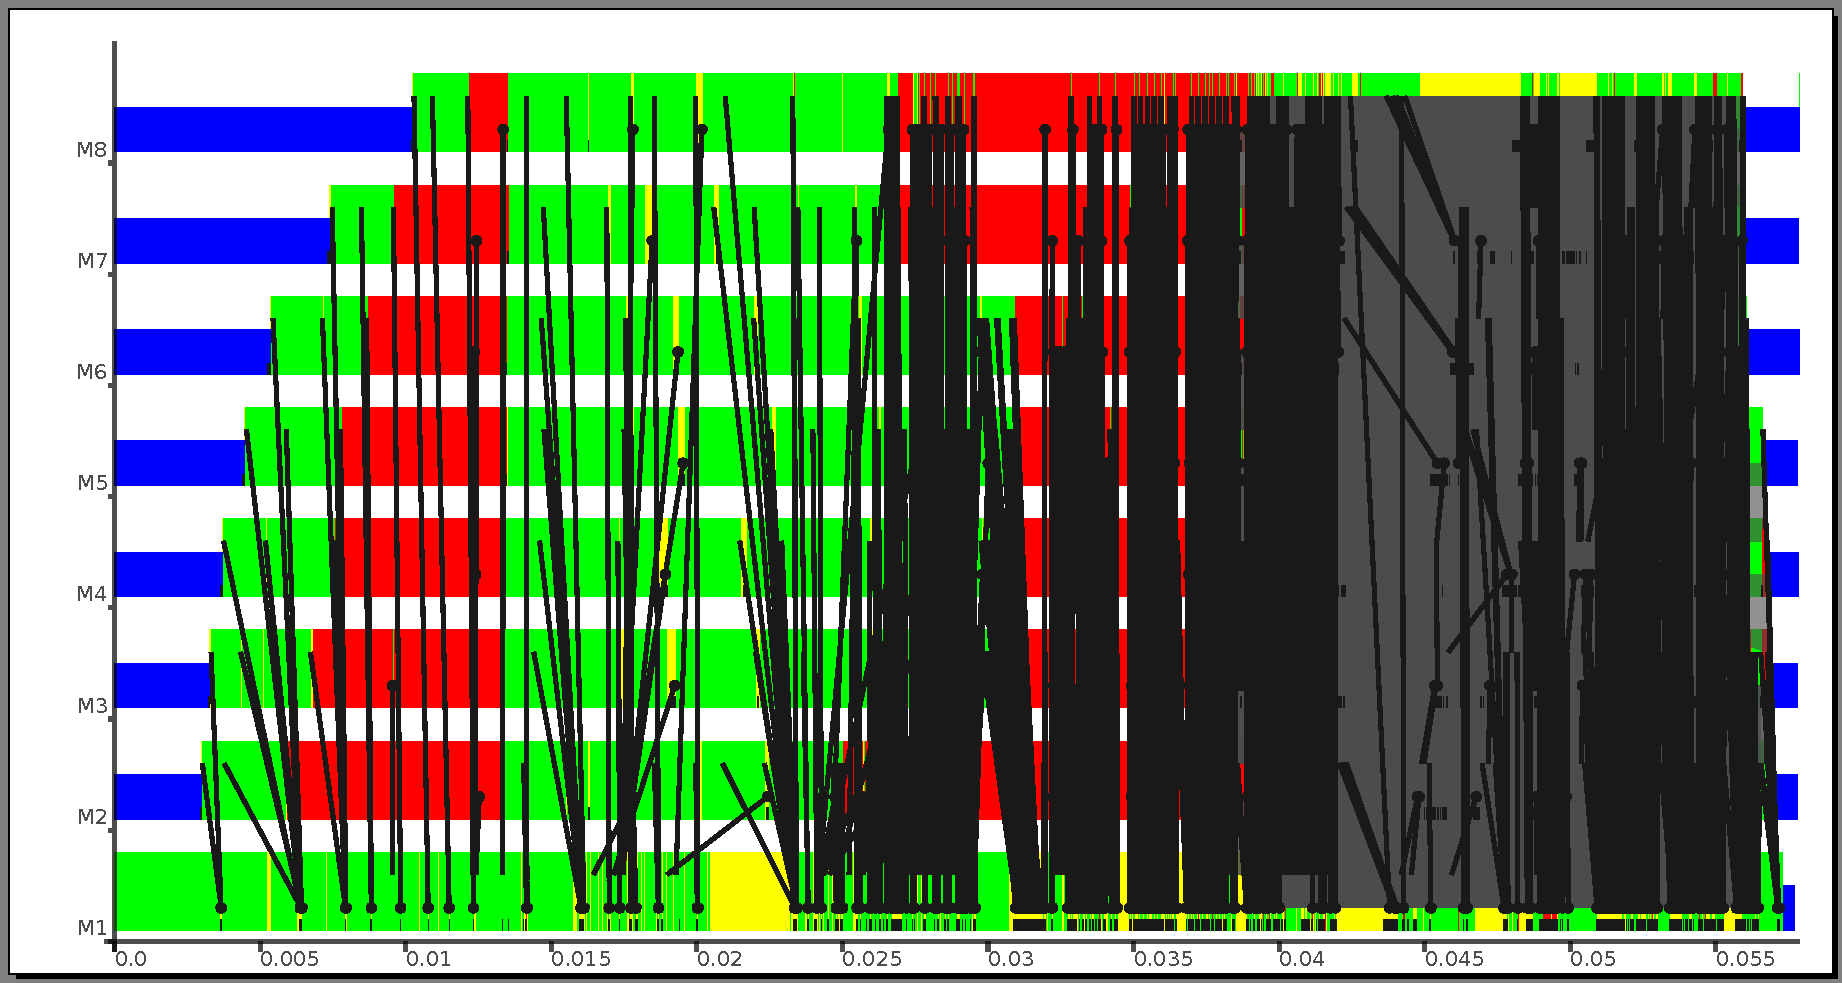
\includegraphics[width=0.9\textwidth]{images/torus_matrix_parrows_scale}
	\caption[Matrix Multiplication with |torus| (PArrows)]{Matrix Multiplication with |torus| (PArrows).}
	\label{fig:torus_parrows_trace}
\end{figure}

\begin{figure}[tb]
	\centering
	\includegraphics[width=0.9\textwidth]{images/torus_matrix_eden_scale}
	\caption[Matrix Multiplication with |torus| (Eden)]{Matrix Multiplication with |torus| (Eden).}
	\label{fig:torus_eden_trace}
\end{figure}

%\FloatBarrier

%%% Local Variables:
%%% mode: latex
%%% TeX-master: "main"
%%% End:
